\documentclass[compress, blue, hyperref={unicode, bookmarks=true, pdfpagemode=FullScreen}]{beamer}
\mode<presentation>
\usetheme{Madrid}
\useoutertheme[subsection=false]{smoothbars}
\beamertemplateshadingbackground{yellow!30}{white}
%\usepackage{tikz}
\usepackage[french]{babel}
\usepackage[utf8]{inputenc} 
\usepackage[T1]{fontenc} 
\usepackage{multicol}
\usepackage{color}
\usepackage{graphicx}
\usepackage[all]{xy}
\usepackage{array}
\setbeamertemplate{navigation symbols}{}


\usepackage{amsmath, amssymb, esint, amstext}
\setbeamertemplate{theorem begin}
{
\begin{\inserttheoremblockenv}
{Th\'eor\`eme}}

\setbeamerfont{frametitle}{size=\large}

\AtBeginSection[] {
  \begin{frame}[t]
    \frametitle{Plan}
      \tableofcontents[sectionstyle=show/shaded,subsectionstyle=hide]
  \end{frame}
} 

\title[SEME 2014]{Projet Axessim : Calcul de matrice d'imp\'edance pour la simulation num\'erique des lignes de transmission multi-conducteur}
\author[Projet Axessim ]{Propos\'e par C. Giraudon, P. Helluy et T. Strub, \\[1ex]
avec J. Aghili, G. Doll\'e, N. Pham, A. Samake, A. Assmar }
\institute[ ]{Semaine d'\'etude Maths-Entreprises
\vspace{.5cm}



\includegraphics[height=1cm]{Logos/unistra.jpg}
\hspace{3cm}

\includegraphics[height=1cm]{Logos/inr}
}
\date{Strasbourg, le 27 juin 2014}

%%%%%%%%%%%%%%                      Debut du document                             %%%%%%%%%%%%%%%


\begin{document}


%%%%%%%%%%%%%%                      Titre                             %%%%%%%%%%%%%%%
\begin{frame}
  \titlepage
\end{frame}





%%%%%%%%%%%%%%                      TOC                             %%%%%%%%%%%%%%%



\begin{frame}[allowframebreaks]
\frametitle{\Large Plan de la pr\'esentation }
\tableofcontents[hideallsubsections]
\end{frame}



%%%%%%%%%%%%%%                      Introduction                             %%%%%%%%%%%%%%%

\section[Intro.]{Introduction}\subsection{hack}
%------------------------------------------------------------------------------
\begin{frame}
  \frametitle{Probl\`eme physique}
  %JE VAIS
  Calculer les tensions $U(z,\omega) =(u_1 \cdots u_N)^T$ et les courants
  $I(z,\omega) = (I_1\cdots I_N)$ complexes dans un faisceau de conducteurs
  $w_i$, $i=1\cdots N$. Les cables sont entour\'es d'un blindage $w_0$. La forme
  du faisceau est fix\'ee dans le plan $(x,y)$ et invariante suivant $z$.
  \begin{center}
    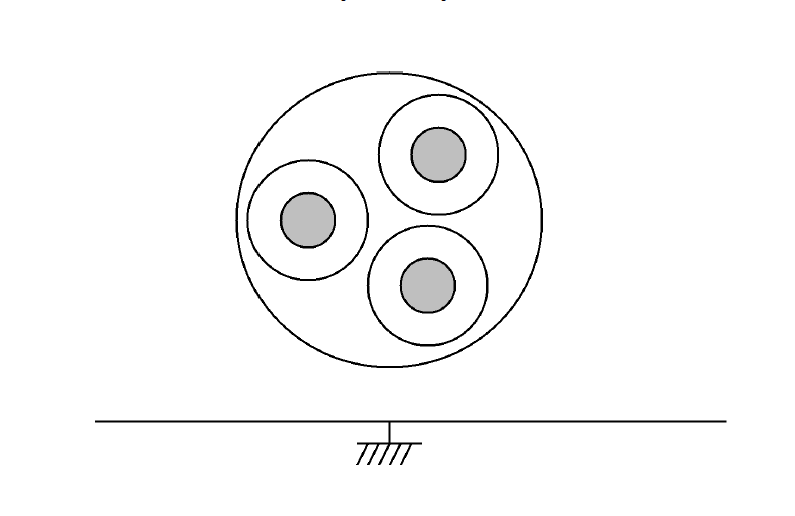
\includegraphics[height=4cm]{figures/f1}\\
    \small  Exemple de section d'un cable.
  \end{center}
\end{frame}
%------------------------------------------------------------------------------


\begin{frame}
\frametitle{Ligne de transmission}
\'Equation des lignes de transmissions ($j^2=-1$)
\begin{eqnarray*}
\frac{\partial U}{\partial z} =ZI, \quad Z=R+j\omega L,\\
\frac{\partial I}{\partial z} =YU, \quad Y=G+j\omega C.
\end{eqnarray*}
Matrices: 
Imp\'edance $Z$, R\'esistance $R$, Inductance $L$, Admittance $Y$, Conductance $G$, Capacit\'e
$C=L^{-1}.$\\[0.4cm]
Propri\'etes des matrices: 
\begin{itemize}
\item Sym\'etrique
\item D\'efinie positive
\end{itemize}

\end{frame} 

\begin{frame}
\frametitle{Probl\`eme}
Flux magn\'etique $\varphi(x,y)$. \\
Champ magn\'etique: d\'erive d'un potentiel vecteur 
$$B=\nabla \times (0,0,\varphi)^T.$$ et
$$\nabla\times B=(0,0,j_z)^T$$ avec
\begin{itemize}
\item  $j_z(x,y)$ : densit\'e de courant suivant $z$
\item  $I_i= \int _{w_i}j_z(x,y)dxdy$ :  courant
\end{itemize}
On a
\begin{equation}
-\Delta\varphi =
\begin{cases}
j_z \\ 
0 \qquad \text{sur } \Omega =w_0 \setminus \cup_i w_i,
\end{cases}
\end{equation} 
\end{frame}



%%%%%%%%%%%%%%                      modèle et assemblage matrice                            %%%%%%%%%%%%%%%


\section[Mtrice]{Probl\`eme}\subsection{prob1}
\begin{frame}
\frametitle{Sous forme de matrice}
%Consid\`ere le mod\`ele
%\begin{equation}
%-\Delta\varphi = j_z 
%\end{equation}
On peut \'ecrire
 \begin{equation}
 \tilde\varphi = \sum_k \phi_k \tilde{\varphi}_k
 \end{equation}
 avec $\tilde{\varphi}$ est solution de probl\`eme suivante 
 \begin{equation}
 \begin{cases}
 -\Delta{\varphi} = 0 \quad \text{sur } \Omega \\
 {\varphi} = \delta_{ij} 
 \end{cases}
 \end{equation}
 donc on a
 \begin{equation}
 \sum_j \phi_j \left( \int_{w_i}-\Delta\tilde{\varphi}_j \right) =I_i
 \end{equation}
 ou bien
 \begin{equation}
  \sum_j \phi_j \left( \int_{\partial w_i}-\nabla\tilde{\varphi}_j \right) \cdot n =I_i
 \end{equation}
 en d'\'eduit
  \begin{equation}
  \sum_j M_{ij}\phi_j =I_i \quad \forall i 
 \end{equation}
%
%\begin{eqnarray*}
%\frac{\partial U}{\partial z} =ZI, \quad Z=R+j\omega L,\\
%\frac{\partial I}{\partial z} =YU, \quad Y=G+j\omega C.
%\end{eqnarray*}


\end{frame} 

 \begin{frame}
\frametitle{Calcul la matrice M}
On a
\begin{equation}
  M_{ij} = \int_{\partial w_j} \frac{\partial\varphi_i}{\partial n}
\end{equation}
 Properties de la matrice $M$
 \begin{itemize}
 \item Sym\'etrique 
 \item D\'efinie positive
 \item Inversible
 \end{itemize}
 Ou bien
\begin{equation}
  M\phi =I \quad \text{ou bien } \phi =LI \quad \text{o\`u } L=M^{-1} 
\end{equation}


\end{frame} 

\begin{frame}
\frametitle{Calcul la matrice M}
Probl\`eme quand on a calculer directement l'int\'egrale : La matrice $M$ n'est plus sym\'etrique 
=> solution: formulation faiblement
\begin{equation}
\int_w -\Delta\varphi \psi =\int_w \nabla\varphi\nabla\psi - \int_{\partial w} \nabla\varphi\cdot n \psi =\int_{\partial w} \nabla\varphi\cdot n 
\end{equation}
avec $\psi \in H^1(w)$ satifait 
\begin{equation}
\psi(z) =
\begin{cases}
0 \qquad \text{ si } z\in w \\
1 \qquad \text{ si } z\in \partial w
\end{cases}
\end{equation} 


\end{frame} 


%%%%%%%%%%%%%%                      assemblage matrice                            %%%%%%%%%%%%%%%


\section[Cabs+blindages]{Cas des cables et des blindages}\subsection{prob2}
%------------------------------------------------------------------------------
\begin{frame}
  \frametitle{Cas des cables et des blindages}
  \begin{columns}[T]
    \column{0.5\linewidth}
    \begin{itemize}
      \item Blindage de r\'ef\'erence $w_0$ et $N$ conducteurs $w_1 \cdots w_N$
      \item Chaque conducteur $w_i$ contient $N^i_{int}$ sous conducteurs
      \item Chaque conducteur $w_i$ matrice d'inductance $L_{int}^i$
      \item $L_{ext}$ : matrice d'inductance des conducteurs ext\'erieurs
    \end{itemize}
    \column{0.5\linewidth}
    \begin{center}
      \begin{tikzpicture}[scale=0.6]
        \draw [thick,fill=cyan!10!white]  (0,0) node (v1) {} ellipse (4 and 4);
        \node at (-4.5,0) {$w_0$};
        \draw [thick,fill=cyan] (-2,0) ellipse (1 and 1);
        \draw [thick,fill=cyan!40!white] (2,0) ellipse (1.5 and 1.5);
        \node at (-2,1.7) {$w_1$};
        \node at (2,1.7) {$w_2$};

        %      \draw [thick,fill=cyan] (2,0) ellipse (0.5 and 0.5);
        \draw [thick,fill=cyan] (2,0.6) ellipse (0.5 and 0.5);
        \draw [thick,fill=cyan] (2,-0.6) ellipse (0.5 and 0.5);
      \end{tikzpicture}
    \end{center}
  \end{columns}
\end{frame}
%------------------------------------------------------------------------------


%------------------------------------------------------------------------------
\begin{frame}
\frametitle{Cas des cables et des blindages}
On obtient
\[ \left[ \begin{array} {c}
\phi_{ext} \\
\tilde{\phi}^1_{int}  \\
\vdots \\
\tilde{\phi}^{N_{int}}_{int} \end{array}  \right]  =
\left[ \begin{array} {cccc}
L_{ext} & & & \\
  & L^1_{int}& &  \\
 & &\ddots &  \\
 & & & L^{N_{int}}_{int} \end{array}  \right]
 \left[ \begin{array} {c}
\tilde{I}_{ext} \\
I^1_{int}  \\
\vdots \\
I^{N_{int}}_{int} \end{array}  \right]
\] \\[0.6cm]
on en d\'eduit
\[ \left[ \begin{array} {c}
\phi_{ext} \\
\tilde{\phi}_{int} \end{array}  \right]  =
\left[ \begin{array} {cc}
L_{ext} & \\
  & L_{int}  \end{array}  \right]
 \left[ \begin{array} {c}
\tilde{I}_{ext} \\
I_{int} \end{array}  \right]
\] \\[0.6cm]
($\tilde{\phi}_{int}$ potentiel int\'erieux calcul\'e avec une r\'ef\'erence sur les blindages)
\end{frame}
%------------------------------------------------------------------------------


%------------------------------------------------------------------------------
\begin{frame}
\frametitle{Cas des cables et des blindages}
Changement de variables
\begin{equation}
\phi_{int} = \tilde{\phi}_{int} +\delta^T \phi_{ext},
\end{equation}
avec $\delta$ : matrice de taille $N_{ext}\times N_{int}$ et
\begin{equation}
\delta(i,j)=
\begin{cases}
1 \qquad \text{si le conducteur $j+N_{ext}$ est dans le conducteur $i$,} \\
0 \qquad \text{sinon.}
\end{cases}
\end{equation}
De plus,
\begin{equation}
\phi_{ext} = L\tilde{I}_{ext}=L(I_{ext}-\delta I_{int})
\end{equation}
La matrice d'inductance globale
\[ \left[ \begin{array} {c}
\phi_{ext} \\
\phi_{int} \end{array}  \right]  =
L
 \left[ \begin{array} {c}
I_{ext} \\
I_{int} \end{array}  \right]
\]
avec
\[ L = P_I^T \left[ \begin{array} {cc}
L_{ext} &0 \\
0 & L_{int} \end{array}  \right] P_I , \qquad
P_I
\left[ \begin{array} {cc}
1 & -\delta \\
0 & 1 \end{array}  \right]
 \]

\end{frame}
%------------------------------------------------------------------------------


%%%%%%%%%%%%%%                      cas test                           %%%%%%%%%%%%%%%


\section[Cas test]{Cas test}\subsection{test}
%-------------------------------------------------------------------------------
\begin{frame}
  \frametitle{Stratégie pour la résolution du problème}
  Plusieurs stratégie possible:
  \begin{itemize}
    \item Méthode intégrale (Choix Axessim)
    \item Méthode élément finis
    \begin{itemize}
    \item Découplage du problème en sous problème simple (Nécessite
      un réassemblage des sous-matrices L et de générer le découpage du maillage).
    \item Résolution du système complet (FreeFEM, Feel++).
    \end{itemize}
  \end{itemize}
\end{frame}
%-------------------------------------------------------------------------------

%-------------------------------------------------------------------------------
\begin{frame}
  \frametitle{G\'en\'eration de conducteurs et maillage}
  \begin{columns}[T]
    \column{.5\linewidth}
    \begin{itemize}
      \item Maillage explicite sur des cas tests simples.
      \item G\'en\'eralisation sur des g\'eom\'etrie contenant des conducteurs
        imbriqu\'e sur diff\'erent niveaux (blindages successifs).
      \item Utilisation d'outils de maillage automatique et param\'etrique (GMSH et FreeFem)
    \end{itemize}
    \column{.5\linewidth}
    \centering
    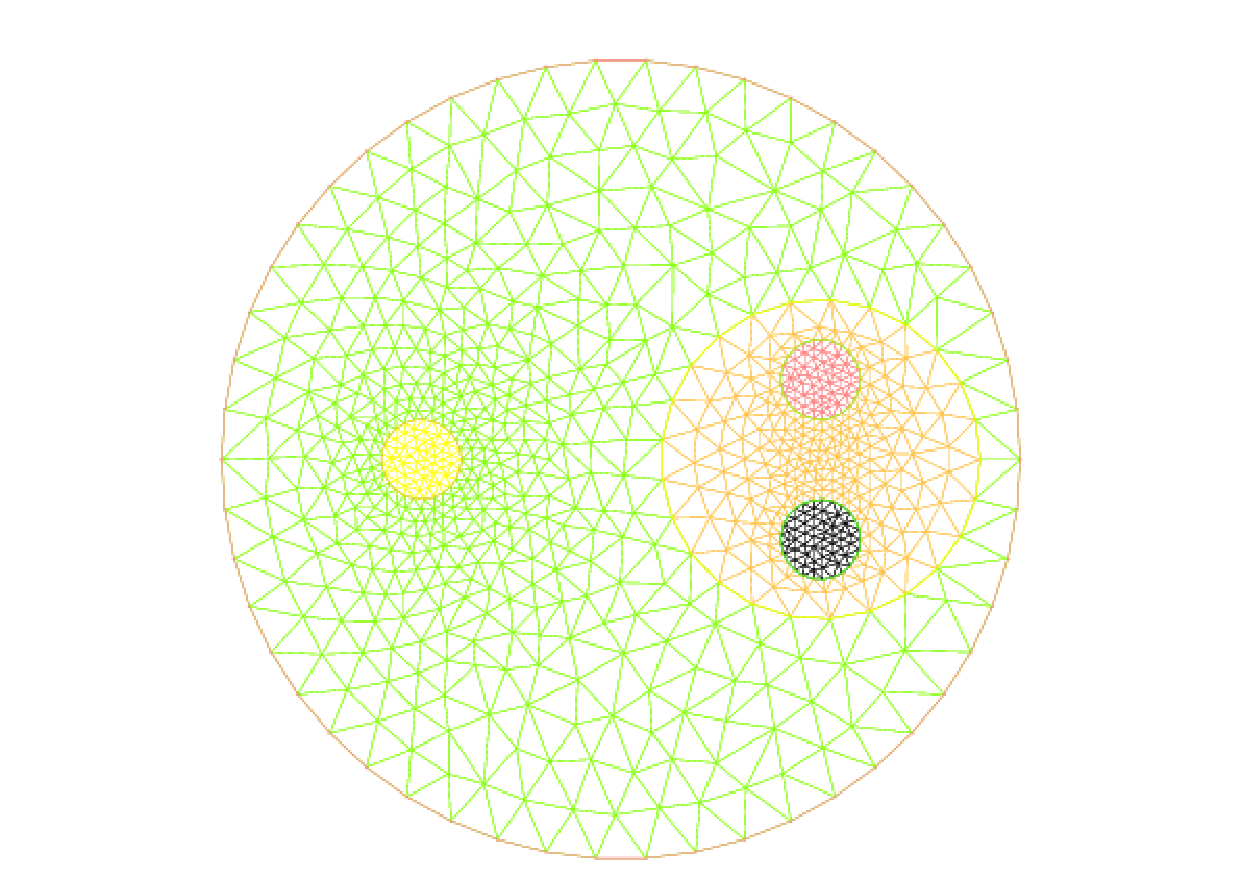
\includegraphics[width=.7\linewidth]{figures/figures/gui/mesh-1.pdf}\\
    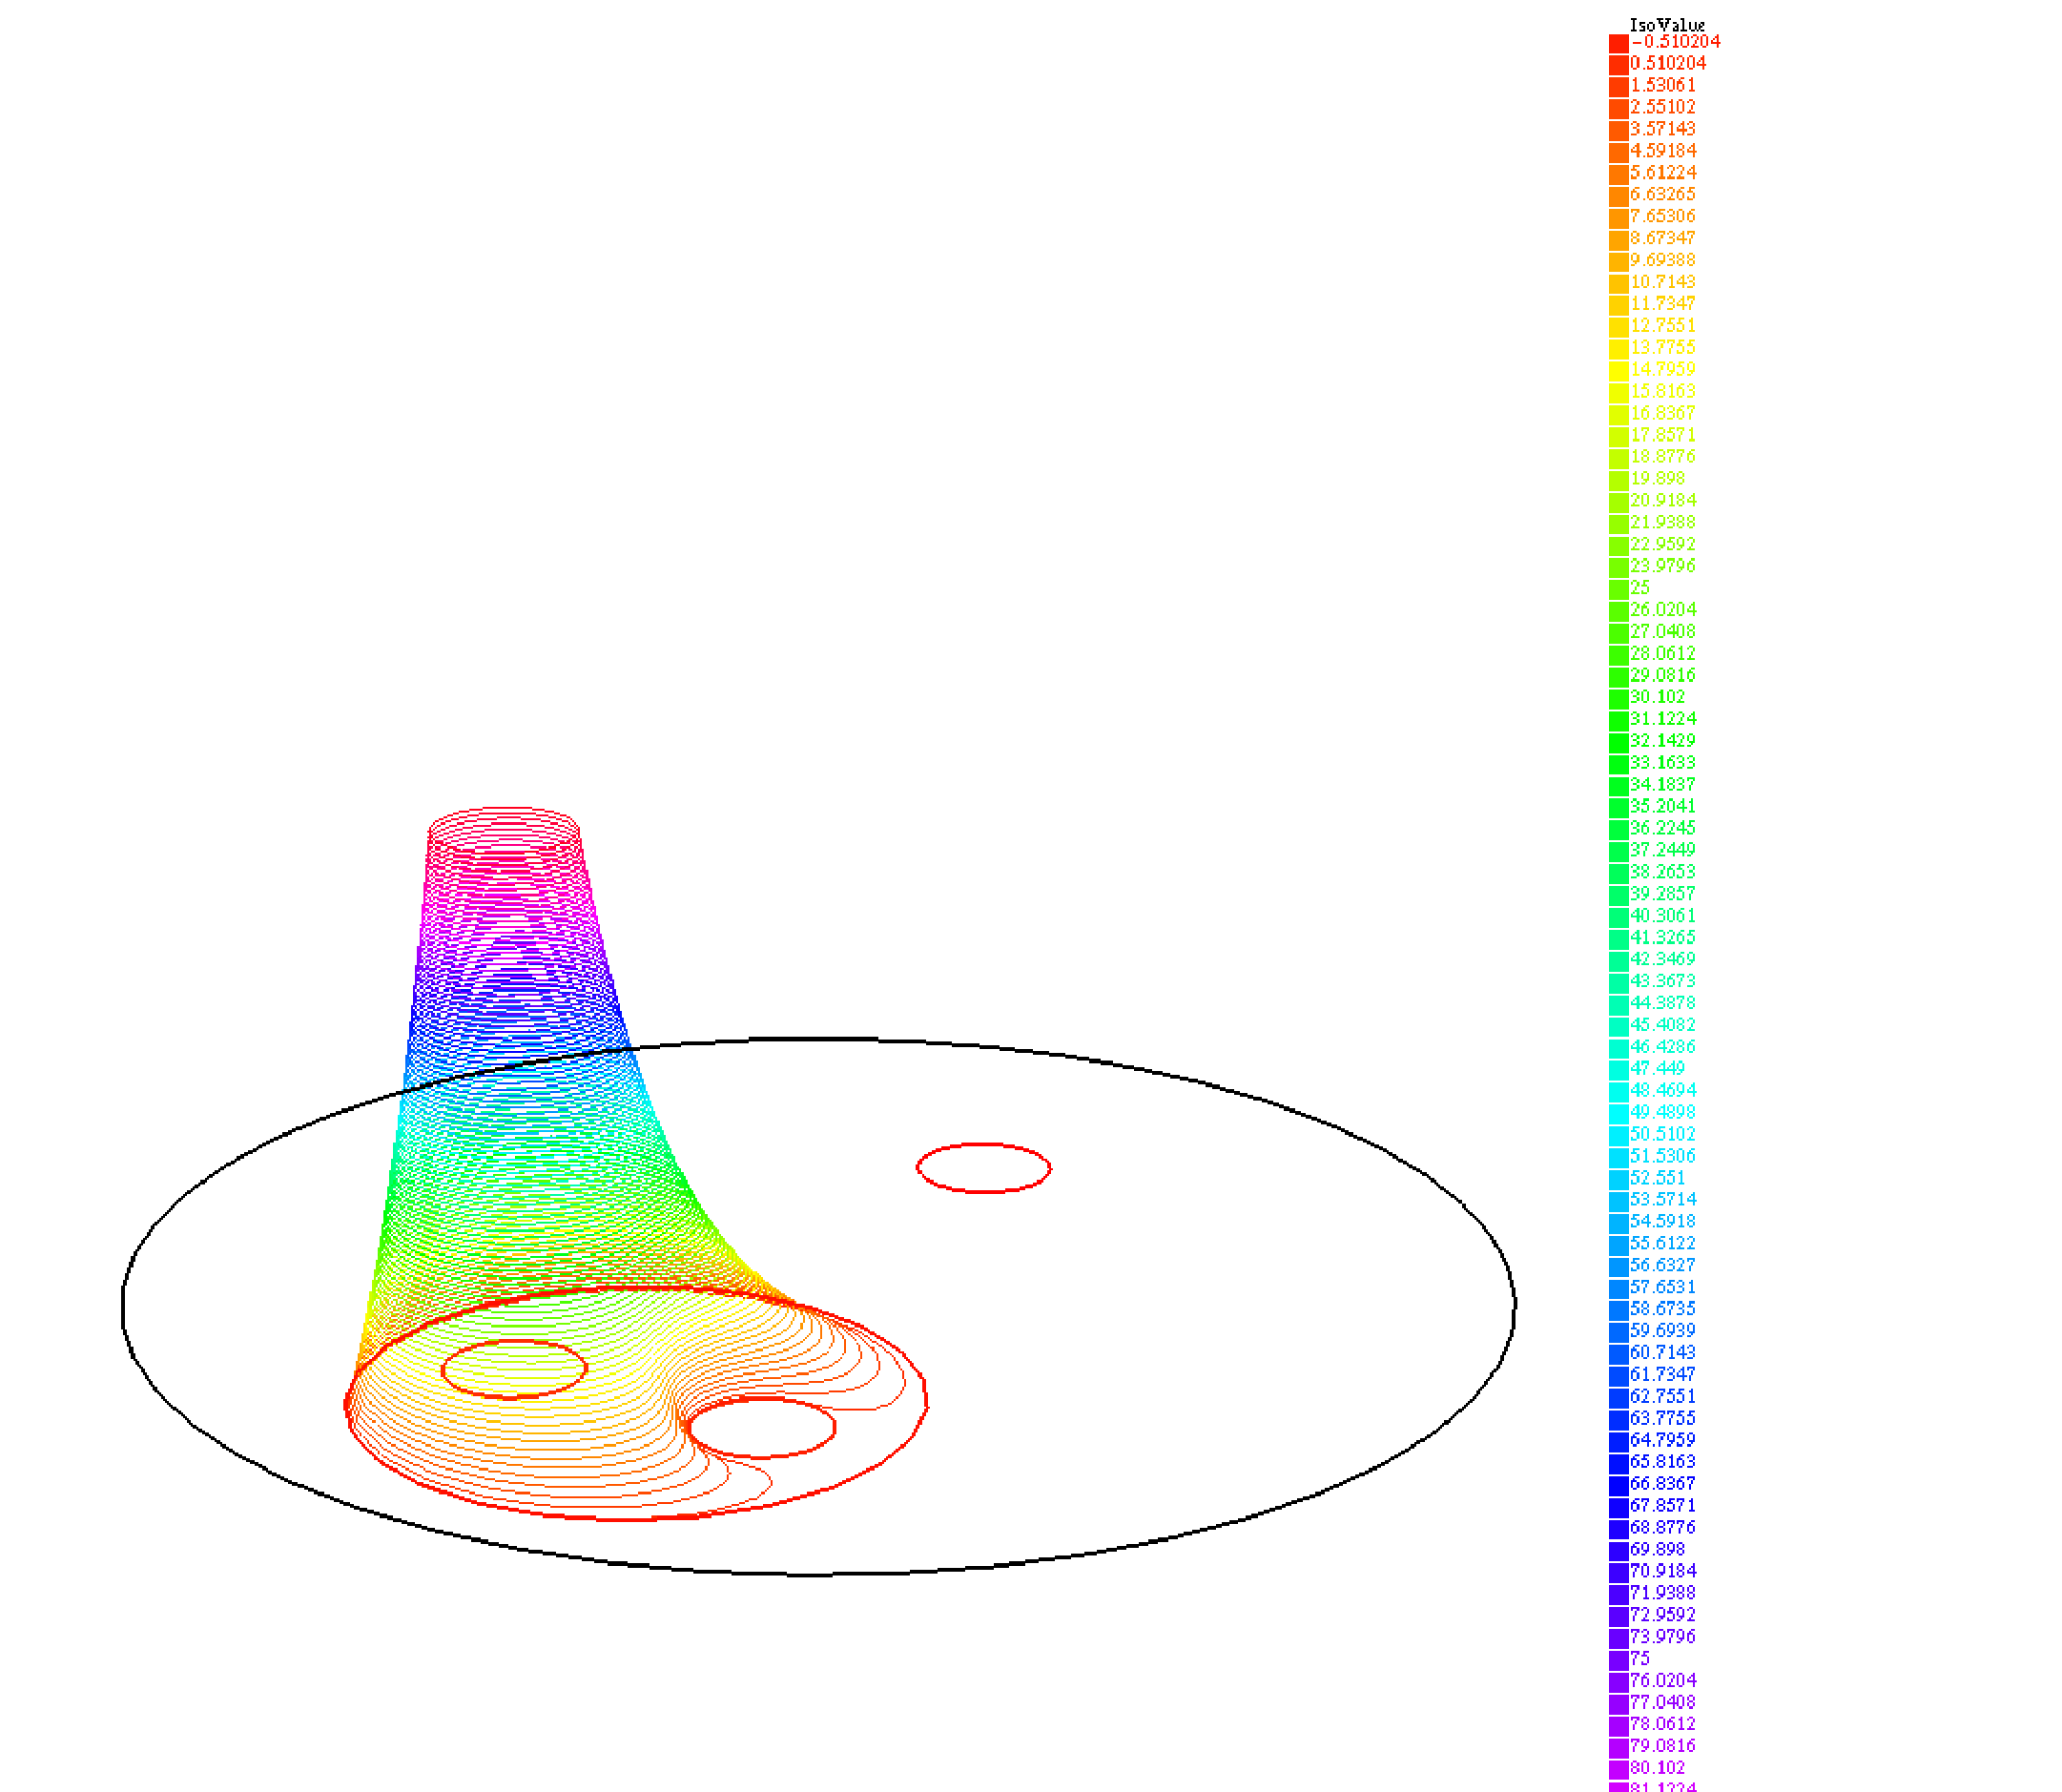
\includegraphics[width=.7\linewidth]{figures/figures/gui/sol3D-1.pdf}
  \end{columns}
\end{frame}
%-------------------------------------------------------------------------------

%-------------------------------------------------------------------------------
\begin{frame}
    \frametitle{Maillage multi-niveaux}
    \begin{columns}[T]
        \column{.5\linewidth}
        \centering
        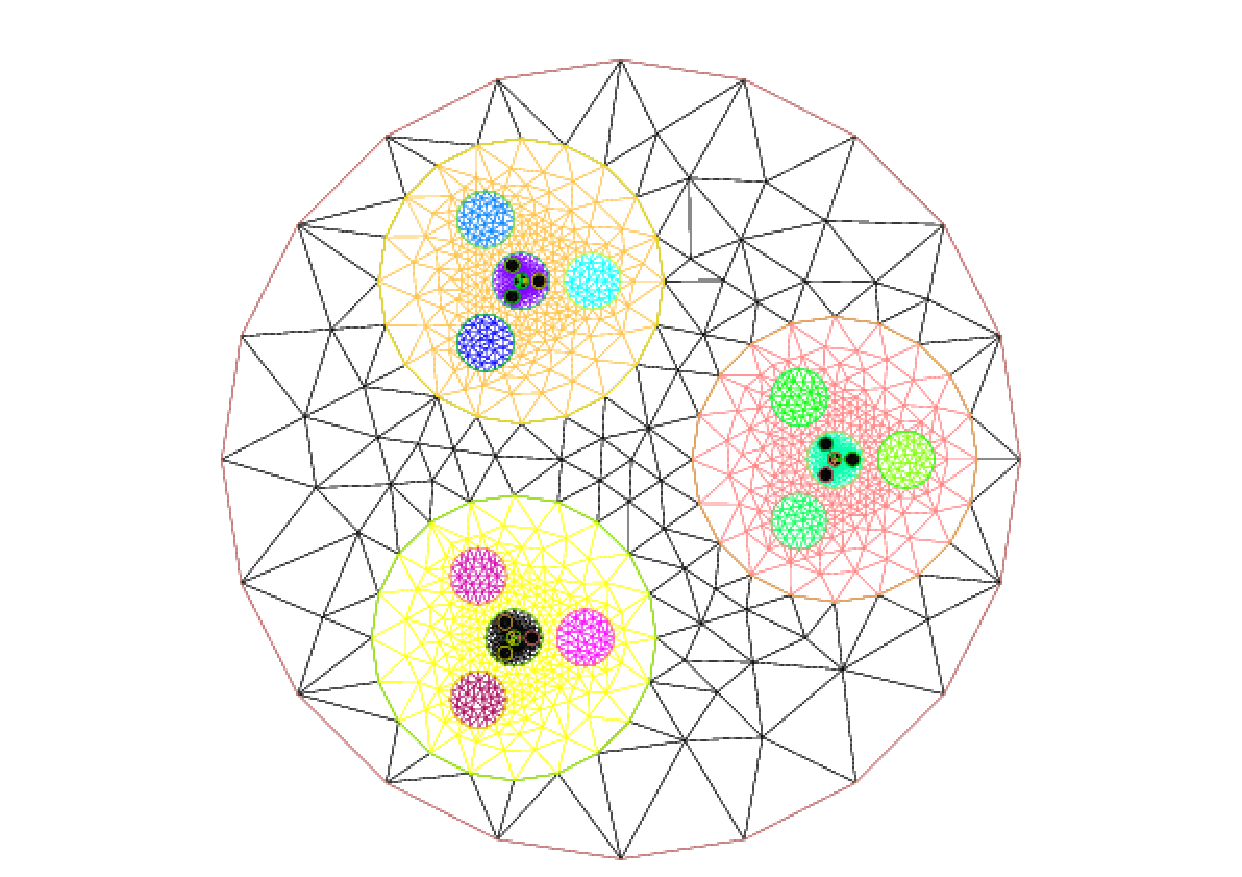
\includegraphics[width=1.2\linewidth]{figures/figures/gui/mesh-2.pdf}
        \column{.5\linewidth}
        Création de différent niveaux de conducteurs par construction itérative:
        \begin{itemize}
            \item Blindage principale extérieur contenant 3 blindages
            \item Chaque sous blindage contient 3 conducteurs et 1 blindage
            \item Répétition des deux précédentes étapes dans les étages inférieurs
        \end{itemize}
    \end{columns}
    L'idée est de retrouver le défaut de positivité qui apparait sur ce genre de géométrie.
\end{frame}
%-------------------------------------------------------------------------------

%-------------------------------------------------------------------------------
\begin{frame}
  \frametitle{Comparaison et difficultés}
  \begin{columns}[T]
      \column{.5\linewidth}
  \begin{itemize}
      \item Découpez chaque niveau de maillage en sous maillage en respectant la numérotation.
      \item Dans le cas du découplage, chaque conducteur est considéré comme un trou sur la
          géométrie.
  \end{itemize}
      \column{.5\linewidth}
  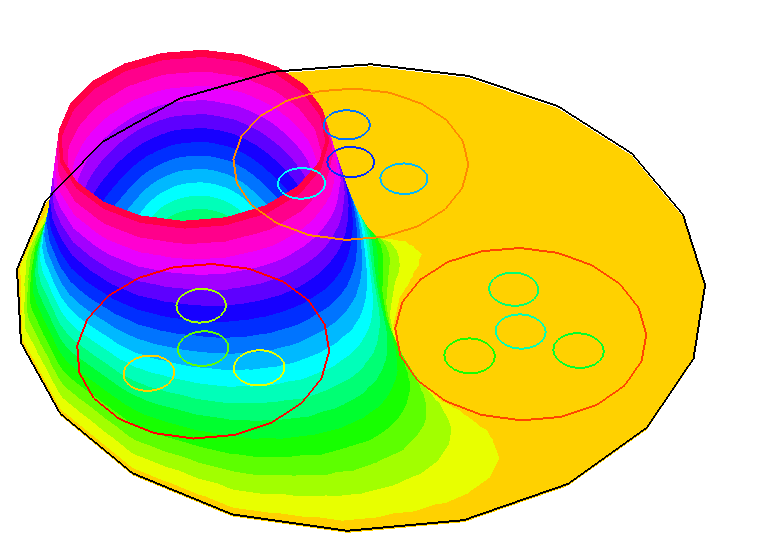
\includegraphics[width=.5\linewidth]{figures/figures/gui/sol3Dfull2-1.png}
  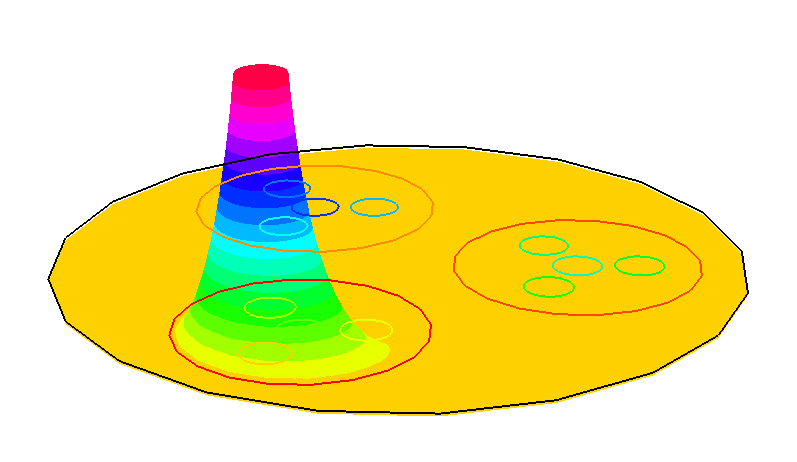
\includegraphics[width=.5\linewidth]{figures/figures/gui/sol3Dfull2-2.png}\\
  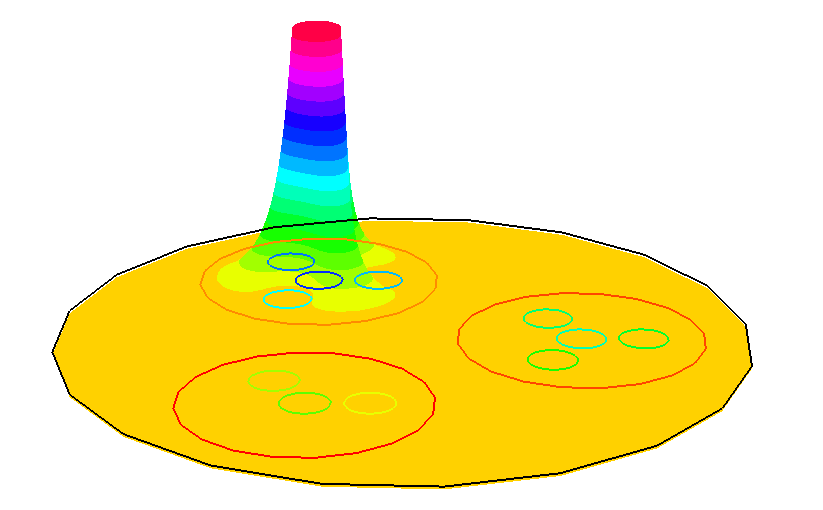
\includegraphics[width=.5\linewidth]{figures/figures/gui/sol3Dfull2-3.png}
  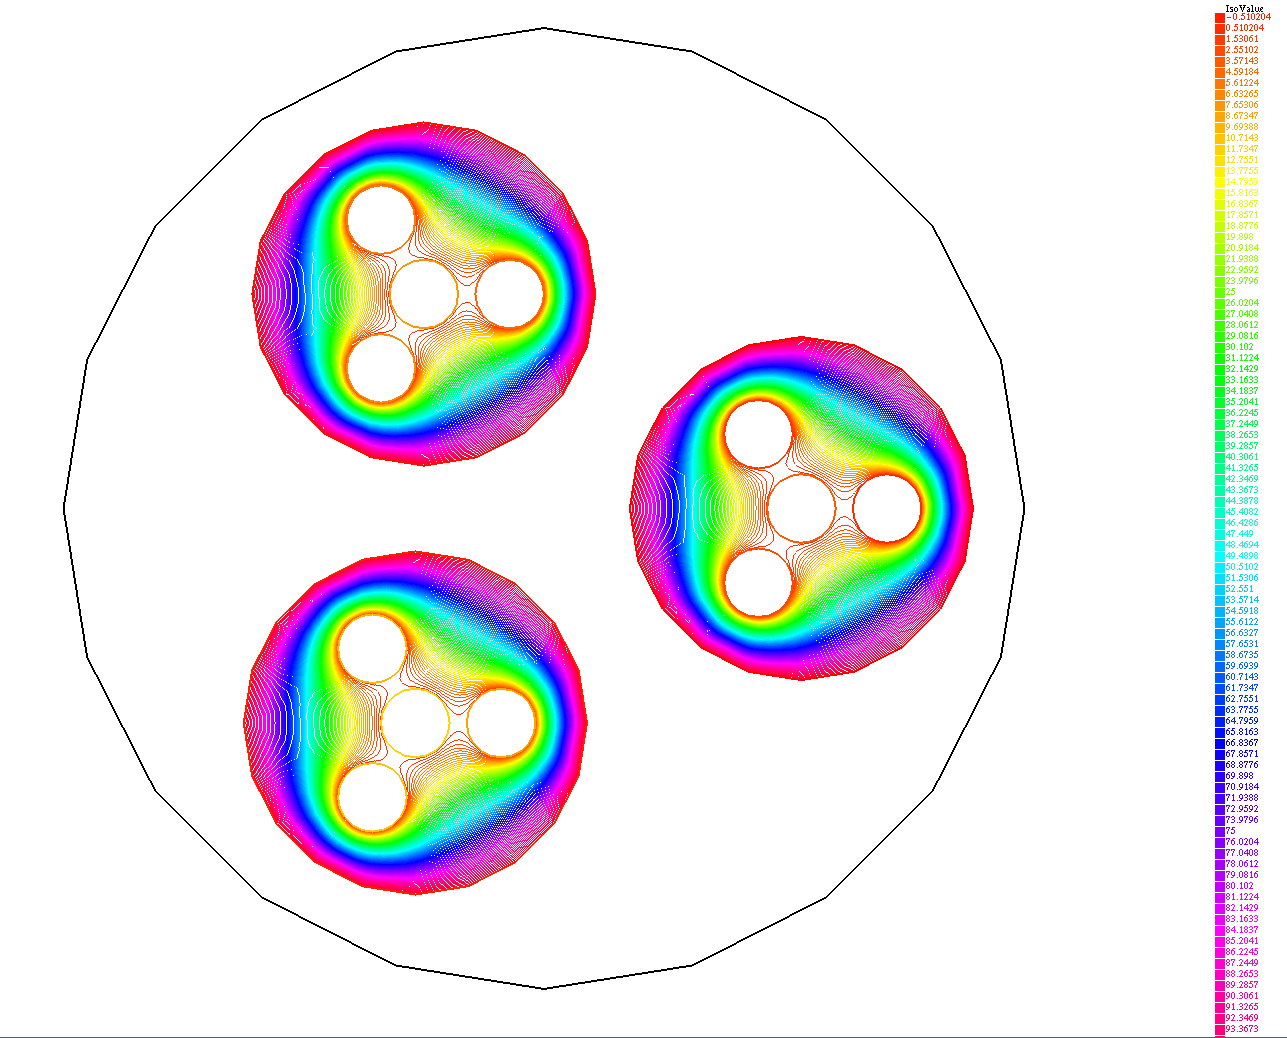
\includegraphics[width=.5\linewidth]{figures/figures/gui/sol3Dfull2-4.png}
  \end{columns}
\end{frame}
%-------------------------------------------------------------------------------

\begin{frame}{Deux niveaux de blindage}
  \begin{figure}[h!tbp]
    \centering
    \subfigure[Niveau 1 de blindage]{\label{level1} 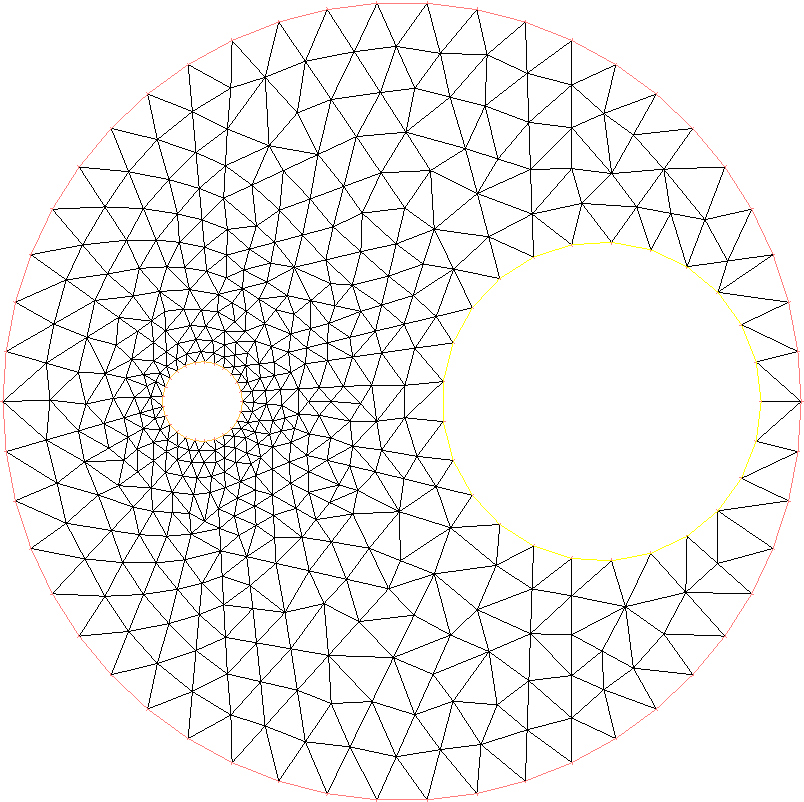
\includegraphics[width=.45\linewidth]{../figs/Th0.pdf}} \hspace{0.5cm}
    \subfigure[Niveau 2 de blindage]{\label{level2} 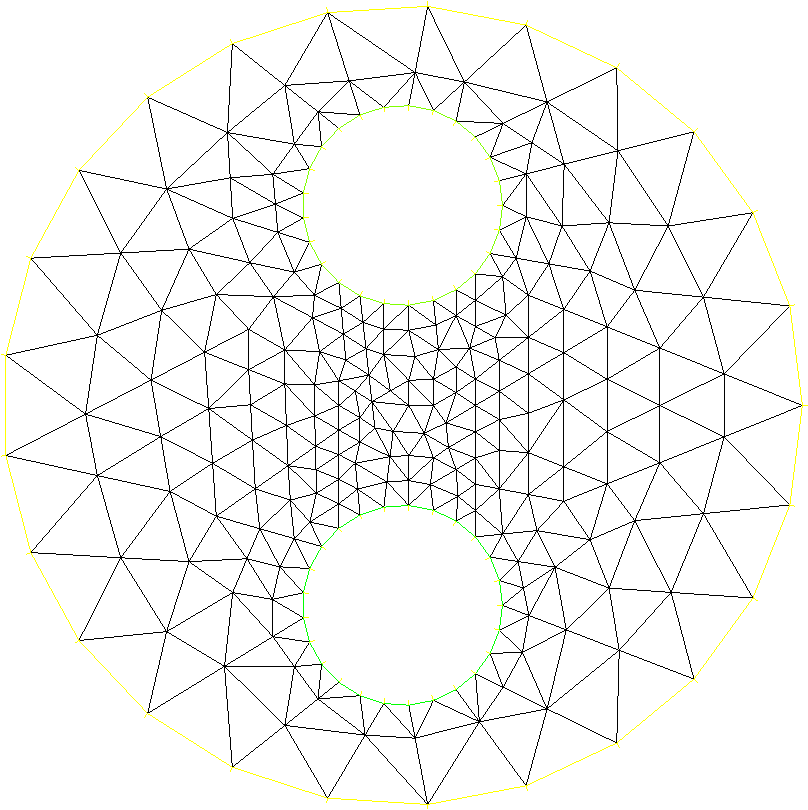
\includegraphics[width=.45\linewidth]{../figs/Th1.pdf}} %\hspace{0.75cm}
    %\subfigure[Trial basis functions in $P_2$]{\label{fig:trial:basis:functions} \includegraphics[width=0.3\linewidth]{basis_trial}}
    % \caption{Basis functions}
    \label{fig:basis:functions}
  \end{figure}
\end{frame}


\begin{itemize}
\item Résolution du problème \ref{eq:2} sur les maillages \ref{level1} et \ref{level2}
\item Assemblage de la matrice de conductivité $M$ présentée dans \ref{eq:3}
\item Calcul de la matrice d'inductance $L=M^{-1}$ présentée dans \ref{eq:4}
\item Vérification des propriétés de la matrice $L$
\end{itemize}

Calcul de la matrice d'inductance global

\Large

\[ L = P_I^T \left[ \begin{array} {cc}
L_{ext} &0 \\
0 & L_{int} \end{array}  \right] P_I , \qquad
P_I=
\left[ \begin{array} {cc}
1 & -\delta \\
0 & 1 \end{array}  \right]
 \]

avec $\delta$ la matrice de taille $N_{ext}\times N_{int}$ définie par

\normalsize
\begin{equation}
\delta(i,j)=
\begin{cases}
1 \qquad \text{si le conducteur $j+N_{ext}$ est dans le conducteur $i$,} \\
0 \qquad \text{sinon.}
\end{cases}
\end{equation}

\begin{frame}
Observation: Le modèle simple à deux niveaux avec peu de cables ne reproduit pas le problème. 

Nécessite d'étudier un problème un peu plus complexe:
%% \begin{figure}
%%   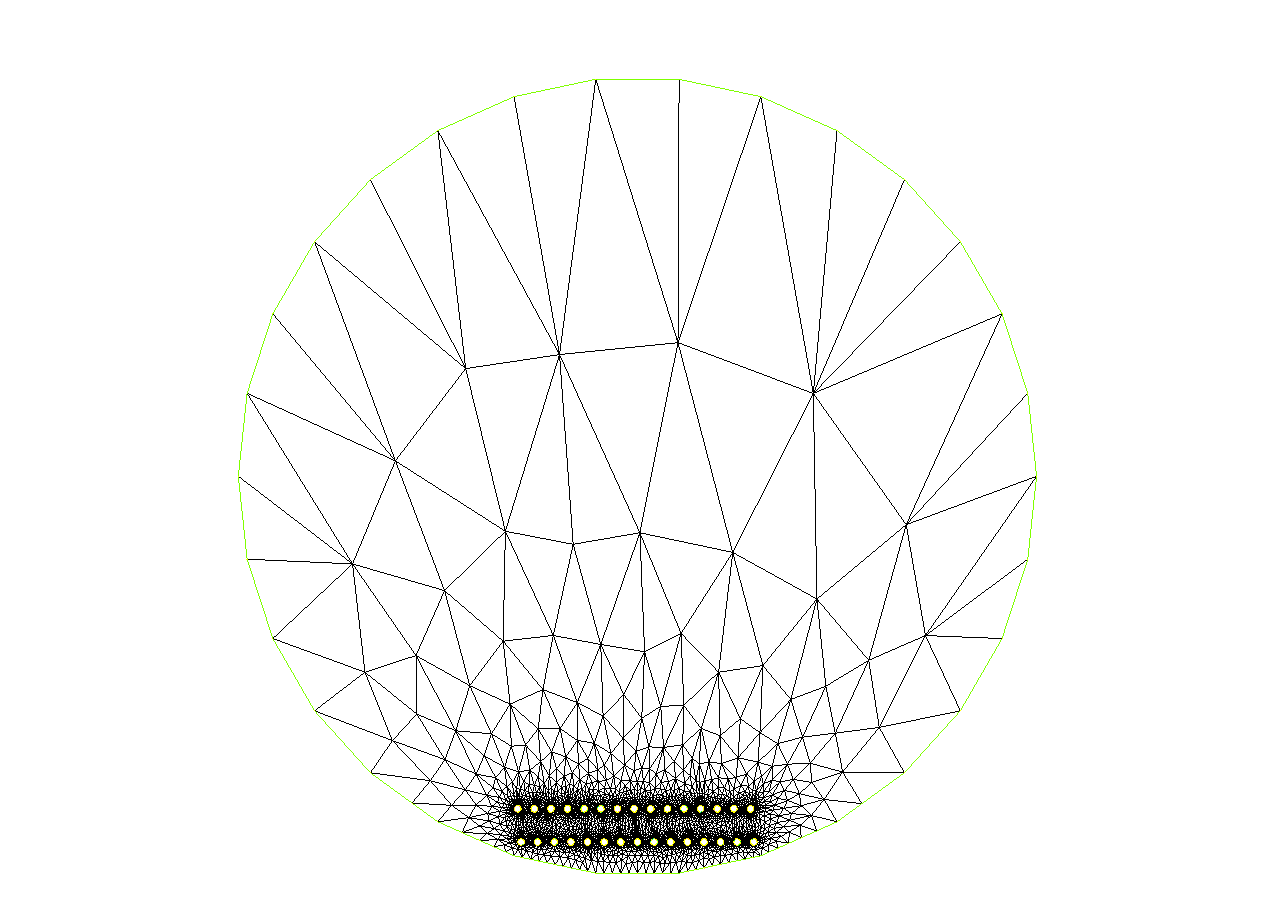
\includegraphics[scale=0.25]{../figs/bigcircle}
%%   \caption{Cas d'un blindage à deux niveaux}
%% \end{figure}
  \begin{figure}
    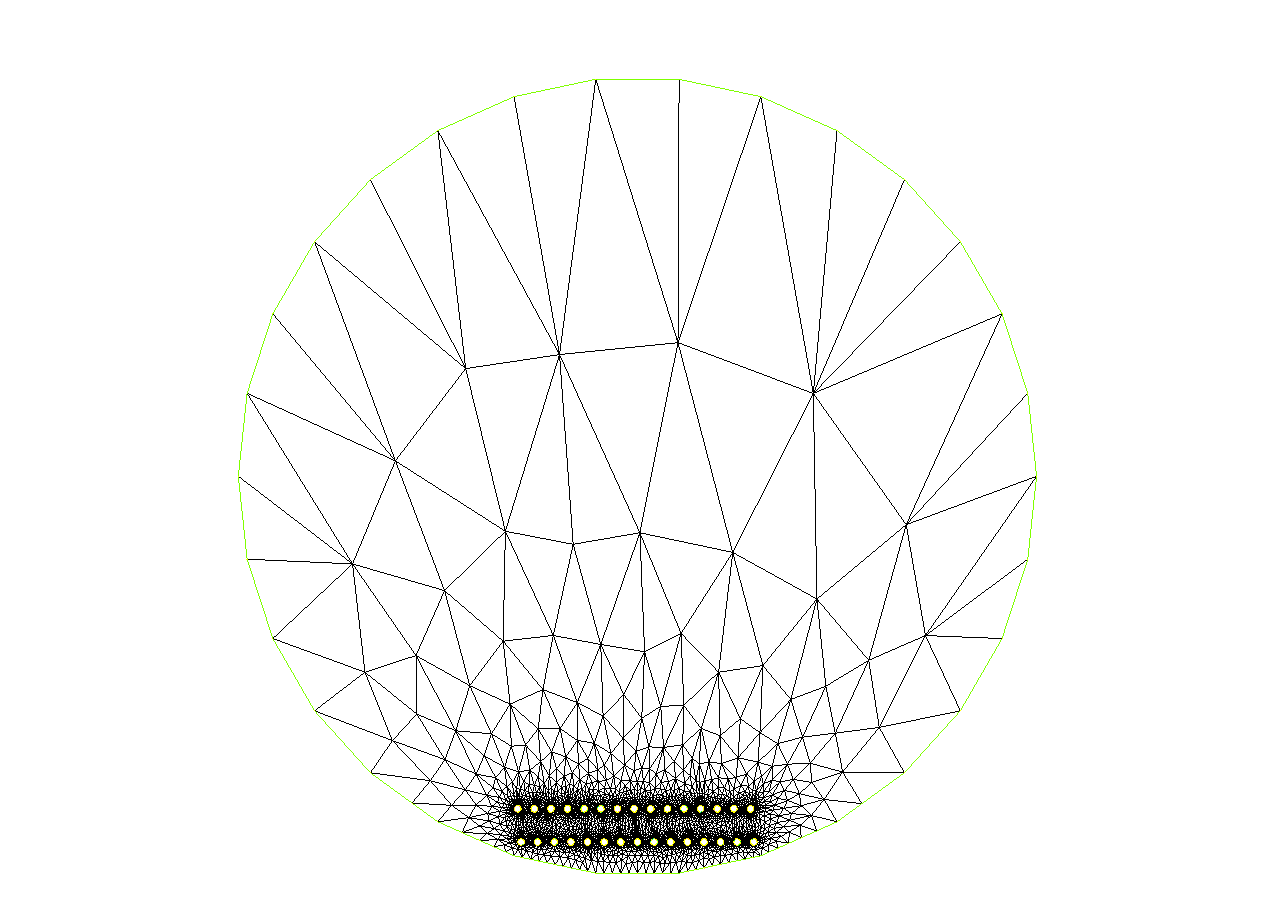
\includegraphics[scale=0.15]{../figs/bigcircle}  \hspace{1pt}
    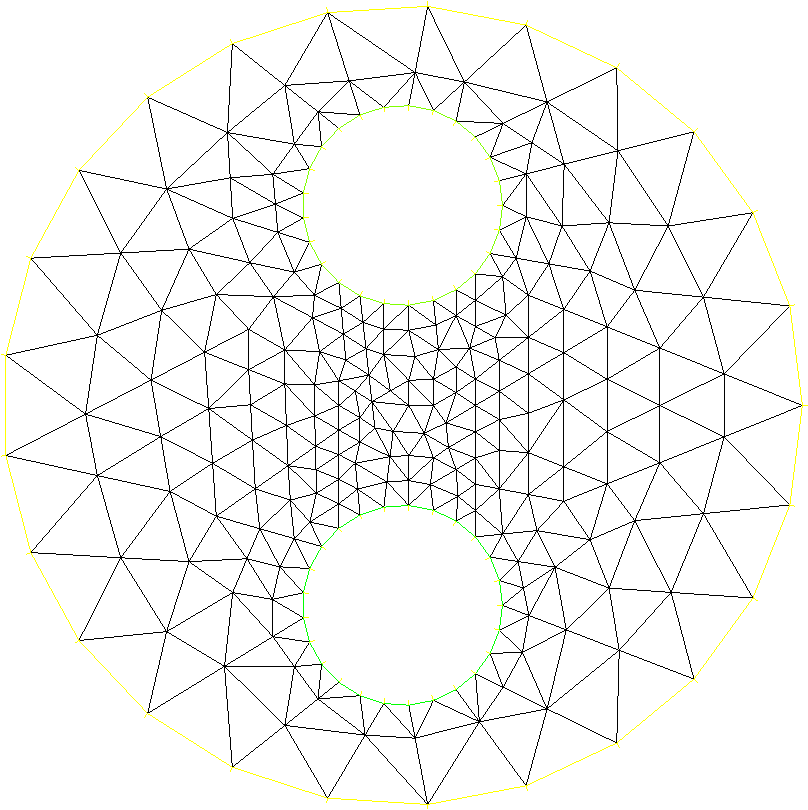
\includegraphics[scale=0.15]{../figs/Th1}  \hspace{1pt}
    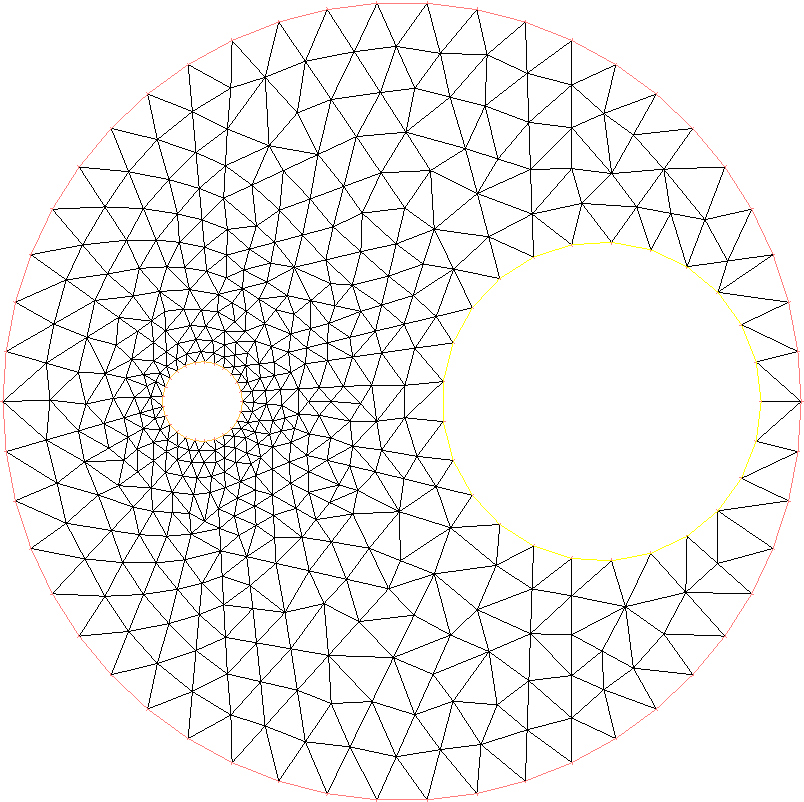
\includegraphics[scale=0.15]{../figs/Th0} \hspace{1pt}    
    \caption{Second blindage à deux niveaux}
  \end{figure}
\end{frame}

\begin{frame}
  \frametitle{Plan d'attaque}
  Procédure d'assemblage:
  \begin{itemize}
  \item Calculer les matrices $M$ du plus bas niveau vers le haut
    \begin{itemize}
    \item Définir la géométrie (FF++) 
    \item $M_{ij}$ nécessite d'introduire une certaine fonction $\psi_j$ localisée autour de $\partial w_j$ (pour obtenir une parfaite symétrie)
    \end{itemize}
  \item Procédures d'inversions de matrices denses ($M \to L$)
  \item Assembler $\delta$ sur le  niveau le plus haut puis la  matrice globale (Non achevé)
  \end{itemize}
\end{frame}

\begin{frame}
\frametitle{Exemple de solution}
TEST
%% \begin{figure}
%%   \includegraphics{../figs/exphi}
%%   \caption{Un exemple de solution du problème de Poisson}
%% \end{figure}
\end{frame}

\begin{frame}
  \frametitle{Observations}
  En pratique, difficultés rencontrées:
  \begin{itemize}
  \item Comprendre la théorie
  \item S'assurer que $M$ est bien symétrique:
    \begin{itemize}
    \item FreeFem++ : Automatisation des conditions aux bords multiples
    \item $\psi_j$ doit être parfaitement localisée: défauts de symétrie constatés dans le cas de simples projections.
    \end{itemize}
  \item Adapter le maillage.
  \end{itemize}
\end{frame}

\begin{frame}
\frametitle{Observations}

\begin{itemize}
  \item A tous les niveaux, $M,L$ ont les propriétés attendues
    \begin{itemize}
      \item Définies positive, $\kappa \simeq 15$
      \item Symétriques
    \end{itemize}
\end{itemize}


\begin{table}
\begin{tabular}{c|c|c|c}
 & Niv.1 & Niv. 2 & Niv.3\\
$M_{\text{ext}}$ & - & -& - \\
$L_{\text{ext}}$ & - & -& - \\
\end{tabular}
\caption{Temps de calculs}
\end{table}

\end{frame}


%%%%%%%%%%%%%%                      Discussions et perspectives                              %%%%%%%%%%%%%%%

\section{Conclusions et perspectives}\subsection{hack}
\begin{frame}
Bilan :
\begin{itemize}
\item AAA
\item BBB
\item CCC
\end{itemize}
\vspace{1cm}
\pause
Perspectives :
\begin{itemize}
\item Cas g\'en\'eral
\item Probl\`eme global -> local
\item Autres 
\item Modèles plus complexes
\end{itemize}
\end{frame}


\begin{frame}
\begin{center}
\Huge Merci de votre attention !
\end{center}
\end{frame}


%%%%%%%%%%%%%%                  References et FIN                                   %%%%%%%%%%%%%%%
\tiny
\include{ref}





\end{document} 



